\chapter{ESTRATÉGIA DE INVERSÃO DO MODELO DE VELOCIDADES}
\label{cap5}

A segunda etapa da estratégia de inversão do modelo de velocidades consiste em encontrar a perturbação
$\delta v$ do modelo de velocidades de background obtido no capítulo anterior.
Esta etapa do desenvolvimento da tese ainda não está totalmente concluída.

\begin{equation}
\label{eq:5.1}
v(x,z)=z g_z+v_0+\delta v
\end{equation}

\begin{figure}[H]
\caption{Representação esquemática do algoritmo de inversão do modelo de velocidades.}
\begin{center}
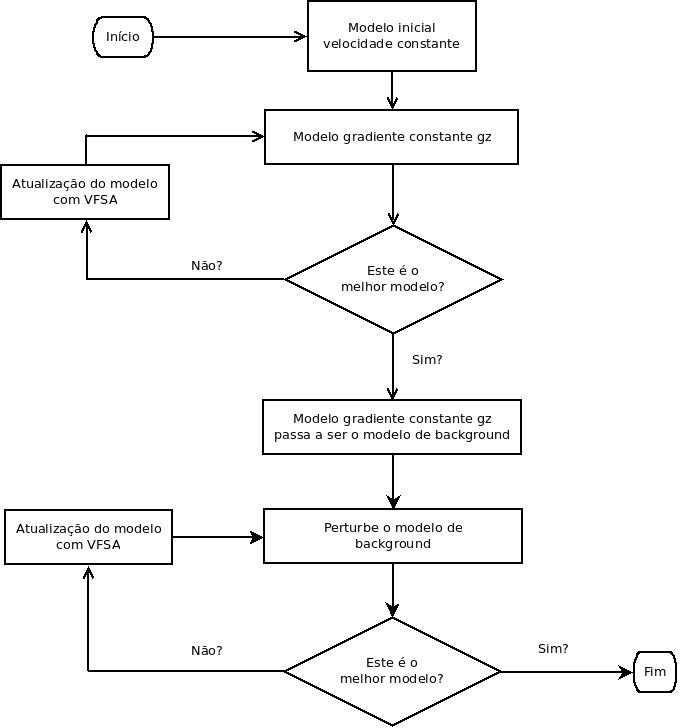
\includegraphics[scale=0.5]{images/fluxonovoVel.jpeg}
\vspace{-0.3cm}
\end{center}
\begin{center}
 Fonte: Do Autor.
\end{center}
\label{fig:5.1}
\end{figure}

O modelo de velocidades é representado pela Equação \ref{eq:5.1} e a
otimização do modelo de velocidades é realizada de forma semelhante à desenvolvida no Capítulo \ref{cap4}:
Utilizamos a Equação \ref{eq:2.2} da soma das diferenças nos tempos de trânsito obtidos com o tratamento de raios no modelo de velocidades e os tempos de trânsito calculados utilizando a fórmula do ERC (Equação \ref{eq:2.1}). Todavia, nesta etapa, o algoritmo Very Fast Simulated Annealing (VFSA) é utilizado para realizar a otimização das perturbações $\delta v$ do modelo de velocidades ao invés do gradiente de velocidades em
profundidade, já obtido na etapa anterior. Estas perturbações são atualizadas a cada iteração do VFSA (Ver a estratégia completa na representação esquemática do algoritmo na Figura \ref{fig:5.1}).

Ainda precisamos escolher a melhor estratégia para a representação do modelo de velocidades
e para a interpolação dos pontos sobre a malha. Temporariamente, utilizamos a representação
do modelo de velocidades em profundidade dividido em faixas de tamanho $\Delta x$.
Cada faixa $\Delta x_j$ possui uma função spline cúbica que varia em profundidade
(1D), esta função representa a variação de velocidade em profundidade dentro da faixa.
Assim, a Equação \ref{eq:5.1} se torna, para os nós das funções spline cúbicas:

\begin{equation}
\label{eq:5.2}
v_ij(\Delta x_j,z_i)=z_i g_z+v_0+\delta v_ij
\end{equation}

Deste modo, a estratégia de inversão do modelo de velocidades consiste em obter
as perturbações $\delta v_ij$ do modelo de velocidades de background (Equação \ref{eq:5.2})
de modo a produzir a melhor localização das fontes PIN sobre os refletores em profundidade.
A velocidade próxima à superfície $v_0$ e o gradiente de velocidades $g_z$ são constantes conhecidas
e definem o modelo de velocidades de background.

\begin{figure}[H]
\caption{Resultado da inversão do modelo de velocidades. Houve considerável melhora na
localização das fontes PIN (cruzes em preto) sobre os refletores em profundidade.}
\begin{center}
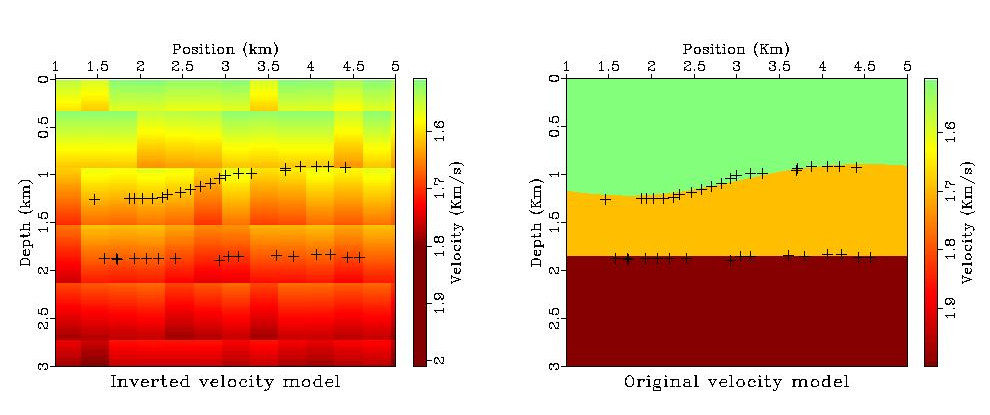
\includegraphics[scale=2]{images/inverted-original.jpeg}
\vspace{-0.3cm}
\end{center}
\begin{center}
 Fonte: Do Autor.
\end{center}
\label{fig:5.2}
\end{figure}

O resultado desta estratégia de otimização do modelo de velocidades é apresentado na Figura \ref{fig:5.2}.
Houve considerável melhora na localização das fontes pontuais PIN sobre os refletores (Ver
Figura \ref{fig:5.2}, à direita) em comparação com a etapa anterior do modelo de velocidades de
gradiente constante (Figura \ref{fig:3.4}).

Estes resultados indicam que a estratégia de inversão do modelo de velocidades utilizada é promissora, porém
que precisa ser elaborada uma melhor estratégia para a interpolação dos pontos sobre a malha do modelo de
velocidades para suavizar o modelo (Figura \ref{eq:5.2}, à esquerda).
